\documentclass[tikz, border=3p]{standalone}
\usepackage{tikz-3dplot}

    \definecolor{deepskyblue}{cmyk}{1,0.25,0.0,0}
    \definecolor{picassoblue}{cmyk}{0.99,0.53,0.0,0.1}
    \definecolor{kelly}{cmyk}{0.59,0,0.64,0.27}
    \definecolor{wales}{cmyk}{0.63,0,0.64,0.21}
    \definecolor{green3}{cmyk}{1,0,1,0.2}
    \definecolor{neonpink}{cmyk}{0,0.57,0.22,0}
    \definecolor{broadwaypink}{cmyk}{0,1,0.5,0} 
    \definecolor{violetflower}{cmyk}{0.25,0.63,0,0}
    \definecolor{darkorcid}{cmyk}{0.25,0.76,0,0.20}

\begin{document}
    \tdplotsetmaincoords{70}{110}    
    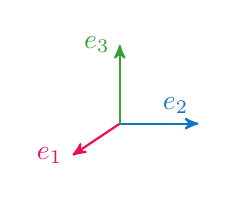
\begin{tikzpicture} [>=stealth',x={(-0.6cm,-0.4cm)}, y={(1cm,0cm)}, z={(0cm,1cm)}, scale=1]   

       

        
             \draw [broadwaypink,thick,->] (0,0) -- (1,0)node[left] {\textcolor{broadwaypink}{$e_1$}};  
             \draw [picassoblue!50!deepskyblue,thick,->] (0,0) -- (0,1)node[anchor=south east] {\textcolor{picassoblue!50!deepskyblue}{$e_2$}}; 
           \begin{scope}[canvas is zx plane at y=0]
             \draw [green3!75!yellow,thick,->] (0,0) -- (1,0) node[left] {\textcolor{green3!75!yellow}{$e_3$}};
             %\draw[top color=deepskyblue!30,fill opacity=.5,deepskyblue] (3,0)--(3,3)--(0,2)--cycle;       
           \end{scope}
    \end{tikzpicture}  

    
\end{document}